\chapter{M\'odulos}
\label{chap:modulos}

%%%%%%%%%%%%%%%%%%%%%%%%%%%%%%%%%%%%%%%%%%%%%%%%%%%%%%%%%%%%%%%%%
%%%%%%%%%%%%%%%%%%%%%%%%%%%%%%%%%%%%%%%%%%%%%%%%%%%%%%%%%%%%%%%%%
\section{Propiedades del sistema}
Estos m\'odulos corresponden principalmente a \textbf{informaci\'on} del set de part\'iculas con el cu\'al se esta trabajando, as\'i como tambi\'en a aquellos m\'odulos que tienen la capacidad de \textbf{modificar} y \textbf{manejar} este set, o alguna propiedad de ellas.
\subsection{cell}
Devuelve informaci\'on del sistema, se utiliza principalmente en \verb|monitor| para entregar esta informaci\'on. \textbf{NO} es necesario cargar este m\'odulo ya que se carga por \textit{default} al correr \lpmd.

\cajatx{
\begin{tabular}{lcl}
 volume & = & Retorna el volumen de la celda.\\
 density & = & Retorna la densidad de la celda.\\
 cell-n & = & n=a,b,c Retorna el largo de cada eje.\\
 particledensity & = & Retorna la densidad por particula. \\
 volumeperatom & = & Retorna el volumen por \'atomo. \\
\end{tabular}
}

\subsection{energy}
Entrega informaci\'on sobre la energ\'ia en el sistema, al igual que \verb|cell|, \textbf{no} es necesario cargar el m\'odulo \verb|energy| ya que es cargo autom\'aticamente al correr \lpmd. La informaci\'on que entrega el m\'odulo a trav\'es de \verb|monitor| es:

\cajatx{
\begin{tabular}{lcl}
 kinetic-energy & = &Retorna el valor de la Energ\'ia \\
                   &&cin\'etica [eV].\\
 potential-energy & = &Retorna la energ\'ia potencial[eV].\\
 total-energy & = &Retorna la energ\'ia total [eV].\\
 momentum & = &Retorna el momentum [uma*A/fs]. \\
 p-n & = &n=x,y,z Retorna el momentum\\
                   && para cada eje. \\
 temperature & = &Retorna el valor de la \\
                 &&temperatura [K].\\
\end{tabular}
}

\subsection{pressure}

Entrega informaci\'on sobre la presi\'on en el sistema y el stress. Este m\'odulo \textbf{SI} es necesario cargarlo antes de llamar a la informaci\'on requerida. Basta llamarlo con,

\control{use pressure \\enduse}

para luego utilizar en \verb|monitor| los llamados posibles de pressure. Es recomendable que primero ``cargue'' el m\'odulo \verb|pressure| y luego especif\'ique el monitor que har\'a menci\'on a alguna de sus propiedades.

\cajatx{
\begin{tabular}{lcl}
 pressure & = & Retorna el valor de la Presi\'on [MPa].\\
 virial-pressure & = & Retorna la contribuci\'on \\
                     &&virial a la presi\'on [MPa].\\
 kinetic-pressure & = & Retorna la contribuci\'on \\
                     &&cin\'etica a la presi\'on [MPa].\\
 sij & = & i,j=x,y,z Retorna los valores del tensor \\
                     &&de stress[MPa]. \\
\end{tabular}
}

%%%%%%%%%%%%%%%%%%%%%%%%%%%%%%%%%%%%%%%%%%%%%%%%%%%%%%%%%%%%%%%%%
%%%%%%%%%%%%%%%%%%%%%%%%%%%%%%%%%%%%%%%%%%%%%%%%%%%%%%%%%%%%%%%%%
\section{M\'odulos Entrada/Salida}
\label{chap:modulos:entradasalida}
Estos m\'odulos pueden ser cargados por \verb|input| y \verb|output|, por lo que los argumentos necesitan ser entregados en esta misma linea. Es decir la instrucci\'on ser\'a siempre de la forma:

\control{input module=nombre opc1=.. opc2=.. ...  opcN=...}

en donde \verb|opcX| son las opciones de cada m\'odulo en paticular. Y de igual forma para \verb|output|.

\subsection{xyz}
\'Este es el m\'odulo que se utiliza para cargar/escribir archivos de configuraci\'on en formato \verb|xyz|, las opciones actuales de este m\'odulo son :

\cajatx{
\begin{tabular}{lcl}
 file & = & archivo de entrada/salida.\\
 level & = & indica el nivel del fichero, estos pueden ser \\
           &&0(pos),1(pos y vel) y 2(pos,vel y ace).\\
 coords & = & utilizado para ``posicionar'' una celda que \\
           &&ha sido leida, sus valores pueden ser \\
           &&centered/uncentered.\\
 inside & = & Puede ser true/false, indica si los \'atomos que \\
          &&est\'an fuera de una celda se deben reubicar.\\
 external & = & ignore/consider. Espec\'ifica si se deben ignorar \\
          &&o considerar los atomos fuera de la celda.\\
\end{tabular}
}

Muchas de estas opciones no son utilizadas en una corrida con \lpmd, sin embargo pueden ser utiles a la hora de trabajar con utilidades tales como \verb|lpmd-analyzer| u otras. En general la forma de utilizar el m\'odulo es,

\begin{itemize}
 \item \textbf{Cargando un fichero xyz}
       \control{input module=xyz file=archivo.xyz}
 \item \textbf{Escribiendo la salida en un fichero xyz con velocidades}
       \control{output module=xyz file=salida.xyz level=1}
\end{itemize}

No todas las opciones son necesarias, muchas de ellas ya tienen valores por defecto, vease \verb|lpmd -p xyz| para m\'as informaci\'on.

\subsection{lpmd}

Es un formato propio de \lpmd, tiene la ventaja de que no s\'olo guarda la informaci\'on de las posiciones at\'omicas de las part\'iculas, sino que adem\'as guarda informaci\'on sobre la celda de simulaci\'on. Las posiciones, a diferencia de \verb|xyz|, se encuentran escaladas, por lo que cuenta con opciones muy simples de manejo, encarecidamente recomendamos su uso para trabajos serios.

\cajatx{
\begin{tabular}{lcl}
 file & = & archivo de entrada/salida.\\
 level & = & indica el nivel del fichero, estos pueden ser \\
           &&0(pos),1(pos y vel) y 2(pos,vel y ace).\\
\end{tabular}
}

La forma com\'un de uso en lpmd es,

\begin{itemize}
 \item \textbf{Cargando un fichero lpmd}
       \control{input module=lpmd file=archivo.lpmd}
 \item \textbf{Escribiendo la salida en un fichero lpmd con velocidades}
       \control{output module=lpmd file=salida.lpmd level=1}
\end{itemize}

\subsection{zlp}

Es un formato similar a \verb|lpmd| sin embargo, este formato utiliza las librerias \textbf{zlib} (para su compilaci\'on), por lo que es un formato binario que utiliza, a diferencia de lpmd, una cantidad de espacio muy reducida en comparaci\'on a los archivos de entrada de tipo \verb|ASCII|.

Las opciones y el uso es similar al formato \verb|lpmd|, salvo algunas opciones de compresi\'on, 

\cajatx{
\begin{tabular}{lcl}
 file & = & archivo de entrada/salida.\\
 level & = & indica el nivel del fichero, estos pueden ser \\
           &&0(pos),1(pos y vel) y 2(pos,vel y ace).\\
 blocksize & = & Tamano del buffer interno de compresi\'on\\
 level & = & Nivel de compresion, 1..6. \\
\end{tabular}
}

La forma de uso, es similar a \verb|lpmd|.

\subsection{crystalfcc}
Genera una celda cristalina del tipo fcc. Este m\'odulo se utiliza en lugar de un fichero de entrada, para entregar las posiciones at\'omicas de la red cristalina, 

\cajatx{
\begin{tabular}{lcl}
 symbol & = & S\'imbolo at\'omico de la especie.\\
 n$\alpha$ & = & $\alpha=x,y,z$ El inverso sobre el largo del cristal.\\
\end{tabular}
}

Consideremos por ejemplo una celda c\'ubica de \textbf{Fe} con un tama\~no de 10 \AA por cada lado.

\begin{itemize}
 \item \textbf{Especificamos el detalle del cristal}
       \control{cell crystall a=10 b=10 c=10 alpha=90 beta=90 gamma=90}
 \item \textbf{Generamos una celda  fcc dentro del cristal}
       \control{input module=crystalfcc symbol=Fe nx=2 ny=2 nz=2}
\end{itemize}

Esto generar\'a entonces una celda cristalina \verb|fcc| para comenzar la simulaci\'on.

\subsection{Otros tipos de crystal}
Al igual que el caso de \textbf{crystalfcc}, existen otros crystales que pueden generarse al comenzar la simulaci\'on, o bien para cualquier otro uso, estos son:
\begin{itemize}
 \item crystalbcc : Generador de redes \verb|bcc|.
 \item crystalsc : Generador de redes \verb|sc|.
 \item crystalhcp : Generador de redes \verb|hcp|.
\end{itemize}

\subsection{crystal2d}
A diferencia de los generadores de cristalprevios, este m\'odulo genera cristales simples bidimensionales, los argumentos requeridos para generar son:

\cajatx{
\begin{tabular}{lcl}
 symbol & = & S\'imbolo at\'omico de la especie.\\
 a & = & Longitud del vector base $\vec{a}$.\\
 b & = & Longitud del vector base $\vec{b}$.\\
 gamma & = & \'Angulo entre los vectores base.\\
 n$\alpha$ & = & $\alpha=x,y$ El inverso sobre el largo del cristal.\\
\end{tabular}
}

Consideremos por ejemplo una celda triangular con atomos de Ar, donde el tamano del cristal es de 10 \AA.

\begin{itemize}
 \item \textbf{Especificamos el detalle del cristal}
       \control{cell crystall a=10 b=10 c=0 alpha=90 beta=90 gamma=90}
 \item \textbf{Generamos una estructura bidimensional dentro del cristal}
       \control{input module=crystal2d a=2 b=2 symbol=Fe gamma=60 nx=2 ny=2}
\end{itemize}

\subsection{skewstart}
M\'etodo creado por \textit{K. Refson} para el c\'odigo de din\'amica molecular \textbf{moldy}. El objetivo del m\'etodo es generar una configuraci\'on no perdi\'odica suficientemente regulr para garantizar una separaci\'on m\'inima entre los \'atomos. Las opciones junto con la forma de generar una celda con \textit{skewstart}, se describe a continuaci\'on:

\cajatx{
\begin{tabular}{lcl}
 symbol & = & S\'imbolo at\'omico de la especie.\\
 atoms & = & Especif\'ica el n\'umero de \'atomos dentro \\
 &&de la celda.\\
\end{tabular}
}

Al igual que los m\'etodos generadores de celda previos, el detalle general del cristal es entregado con la orden \verb|cell|, y el resto specificadio por el m\'odulo, consideremos una cleda de arg\'on de 108 \'atomos con un tamano de 20 \AA y que inicializacmos las posiciones at\'omicas con el m\'etodo \textit{skewstart}

\begin{itemize}
 \item \textbf{Especificamos el detalle del cristal}
       \control{cell crystall a=20 b=20 c=20 alpha=90 beta=90 gamma=90}
 \item \textbf{Generamos una celda  fcc dentro del cristal}
       \control{input module=skewstart symbol=Ar}
\end{itemize}

\subsection{dlpoly}
Este plugin, pretende dar una soluci\'on tipica y eficiente a los archivos de entrada que el usuario ya posee en \verb|dlpoly| y que el trabajo de migrar estos archivos a otras configuraciones podria implicar una inversion de tiempo.

Con el m\'odulo \verb|dlpoly|, se pueden cambiar los archivos de configuracion cristalina de \verb|dlpoly| a cualquier otro m\'odulo y viceversa. Los argumentos utilizados por el m\'odulo \verb|dlpoly| son:

\cajatx{
\begin{tabular}{lcl}
 file & = & Archivo que contiene la configuraci\'on \\
 &&de \textbf{dlpoly}\\
 level & = & Nivel del archivo (0,1,2).\\
 preiodicity & = & Especifica \textit{key} de periodicidad del \\
 &&fichero CONFIG.\\
\end{tabular}
}

\subsection{vasp}
El plugin, es utilizado para leer ficheros POSCAR de \verb|vasp| como un fichero de configuracion inicial, o bien para otro prop\'osito, entre las opciones del m\'odulo, estan:

\cajatx{
\begin{tabular}{lcl}
 file & = & Archivo que contiene la configuracion de \textbf{dlpoly}\\
 species & = & lista de las especies (en orden) del fichero \\
 &&POSCAR.\\
 type & = & Tipo de posiciones, direct/cartesian.\\
\end{tabular}
}
%%%%%%%%%%%%%%%%%%%%%%%%%%%%%%%%%%%%%%%%%%%%%%%%%%%%%%%%%%%%%%%%%
%%%%%%%%%%%%%%%%%%%%%%%%%%%%%%%%%%%%%%%%%%%%%%%%%%%%%%%%%%%%%%%%%
\section{Modificadores}
\subsection{tempscaling}

Utilizado para controlar y escalar la temperatura de la muestra, utilizando rescalamiento de velocidades en las part\'iculas. \'Este es uno de los m\'etodos m\'as utilizados en muchos c\'odigos de din\'amica molecular.

El escalamiento consiste en modificar las velocidades at\'omicas cada cierto intervalo, en un factor:

$$s=\sqrt{\frac{gk_BT}{2\mathcal{K}}}$$

Es importante tener en cuenta, qu el proceso de control o escalamiento de la temperatura, no entregan promedios termodin\'amicos reales, es necesario que estos sean evaluados luego de haber realizado el escalamiento.

Consideremos ahora un ejemplo de utilizaci\'on del m\'odulo \textbf{tempscaling}, en donde calentamos una muestra de Ar a 300K y luego mantenemos la temperatura fija durante un peri\'odo de tiempo, para finalmente liberar el sistema:

En primer lugar debemos cargar los modulos para cada una de las etapas de la simulaci\'on:

\begin{itemize}
 \item \textbf{Cargamos el proceso de calentamiento de la muestra.}
       \control{use cellscaling as uptemp \\   from 84.0\\   to 300.0\\enduse}
 \item \textbf{Cargamos un proceso para mantener la temperatura fija.}
       \control{use cellscaling as fixtemp \\   from 300.0\\   to 300.0\\enduse}
\end{itemize}

Ahora, que el m\'odulo fue cargado, es necesario, en la parte final del archivo de control, especificar entre que intervalos de tiempo van a ser aplicados estos escalamientos:

\begin{itemize}
 \item \textbf{Aplicamos \textbf{uptemp} desde 1 hasta 10000, cada 50 pasos.}
       \control{apply uptemp start=1 end=10000 each=50}
 \item \textbf{Mantenemos la temperatura fija entre 10000 y 15000.}
       \control{apply fixtemp start=10000 end=15000 each=50}
\end{itemize}

De esta forma entonces hemos conseguido una muestra a 300K de temperatura con un proceso de \textit{calentamiento} de la celda inicial.

\subsection{berendsen}
\'Este m\'odulo controla o escala la temperatura, al igual que \textbf{tempscaling}, su diferencia es que el m\'etodo es un escalamiento menos \textbf{brusco}, por lo que en ocaciones se consiguen muy buenos resultados y se logra termalizar de manera m\'as eficiente las muestras. Los argumentos requeridos por el m\'odulo son:

\cajatx{
\begin{tabular}{lcl}
 from & = & Desde que temperatura comenzar a aplicar.\\
 to & = & Temperatura final a la que se desea llegar.\\
 tau & = & Intervalo del termostato.\\
\end{tabular}
}

\textbf{Berendsen} puede aplicarse de igual forma que \verb|tempscaling|.

\subsection{cellscaling}
\'Este m\'odulo es un modificador de la celda, en particular, tiene la propiedad de cambiar el tama\~no de la celda durante la simulaci'on, lo que lo hace una herramienta muy util para ver, por ejemplos, comportamiento de materiales bajo distintas densidades durante una sola simulaci\'on. El m\'odulo tiene las siguientes opciones:

\cajatx{
\begin{tabular}{lcl}
 percent & = & Especifica el porcentaje en el que se variar\'a \\
 &&el largo de la celda.\\
 axis & = & Indica, el eje (x,y o z) en el que se comprimira \\
 &&la celda (all=hidrost\'atico).\\
 constant & = & true/false indica si la modificacion es constante \\
 &&respecto al valor inicial.\\
\end{tabular}
}

Para un detalle m\'as acabado en el uso de cellscaling, vea el cap\'itulo~\ref{chap:exa}.

\subsection{displacement}
M\'odulo que modifica las posiciones at\'omicas del sistema, a partir de un desplazamiento vectorial de los \'atomos de la muestra. Su funcionalidad esta enfocada principalmente en la construcci\'on de sistemas nanoestructurados a futuro.

\cajatx{
\begin{tabular}{lcl}
 x & = & Desplazamiento en el eje x.\\
 y & = & Desplazamiento en el eje y.\\
 z & = & Desplazamiento en el eje z.\\
\end{tabular}
}

\subsection{rotate}
M\'odulo que modifica las posiciones, rotando los \'atomos cierto grado en torno a un origen. Al igual que el m\'odulo \verb|displace|, est\'a desarrollado para la futura creaci\'on de estructuras m\'as complejas.

\cajatx{
\begin{tabular}{lcl}
 x & = & Coordenada x del eje de rotaci\'on.\\
 y & = & Coordenada y del eje de rotaci\'on.\\
 z & = & Coordenada z del eje de rotaci\'on.\\
 angle & = & \'Angulo de rotaci\'on en grados.\\
\end{tabular}
}

\subsection{quenchedmd}
M\'odulo que m\'inimiza la estructura, utilizando el m\'etodo \textit{Quenched Molecular Dynamics}. Durante el proceso, el integrador no actua, como una din\'amica molecular simple, ya que erifica la proyeccion entre fuerza y velocidad, la que se ve forzada si la energ\'ia es incrementada.

El m\'odulo no necesita argumentos especiales, solo ser llamado y aplicado.

%%%%%%%%%%%%%%%%%%%%%%%%%%%%%%%%%%%%%%%%%%%%%%%%%%%%%%%%%%%%%%%%%
%%%%%%%%%%%%%%%%%%%%%%%%%%%%%%%%%%%%%%%%%%%%%%%%%%%%%%%%%%%%%%%%%
\section{Manejadores de Celda}
Estos m\'odulos son los encargados de generar las \textbf{lista inteligentes} para poder realizar simulaciones o c\'alculos de Din\'amica Molecular, los dos plugins implementados a la fecha son:

\subsection{minimumimage}
Uiliza el m\'etodo de m\'inima imagen para realizar los procesos. Es mucho m\'as lento que el m'etodo linkedcell, pero en el s'olo se necesita ingresar el radio de corte del sistema. Est\'e m\'etodo no es bueno cuando el radio de corte es del orden del tama\~no de la mitad de la celda de simulaci\'on.

\begin{itemize}
 \item \textbf{Cargando el M\'odulo}
       \control{use minimumimage \\ cutoff 2.0 \\enduse}
 \item \textbf{Aplicando el M\'odulo}
       \control{cellmanager minimumimage}
\end{itemize}

Con \'esto nuestra simulaci\'on utilizar\'a el m\'etodo de m\'inima imagen para un \verb|cutoff| de 2.0 \AA.

\subsection{linkedcell}
Utiliza el m\'etodo de listas linkeadas, \'este m\'etodo es mucho m\'as rapido que el m\'etodo de m\'inima imagen, y de por s\'i es el m\'as utilizado en la mayor\'ia de los c\'odigos de \textbf{DM}, se puede subdividir la celda a voluntad, sin embargo es recomendable que el tama\~no de subdivisi\'on de la celda no sea menor que la distancia m\'inima de interacci\'on entre las part\'iculas, con algun potencial.

\begin{itemize}
 \item \textbf{Cargando el M\'odulo}
       \control{use linkedcell \\ cutoff 2.0 \\ nx 10\\ ny 10\\ nz 10\\enduse}
 \item \textbf{Aplicando el M\'odulo}
       \control{cellmanager linkedcell}
\end{itemize}

As\'i subdividimos la celda en una grilla de 10x10x10. Para generar las listas de vecinos de cada \'atomo.
%%%%%%%%%%%%%%%%%%%%%%%%%%%%%%%%%%%%%%%%%%%%%%%%%%%%%%%%%%%%%%%%%
%%%%%%%%%%%%%%%%%%%%%%%%%%%%%%%%%%%%%%%%%%%%%%%%%%%%%%%%%%%%%%%%%
\section{Potenciales Interat\'omicos de pares}
\subsection{lennardjones}
El m\'odulo \textbf{lennardjones} hace referencia al potencial de Lennard-Jones, que es de la forma,
$$U(r_{ij}) = 4\epsilon\left(\left(\frac{\sigma}{r_{ij}}\right)^{12}-\left(\frac{\sigma}{r_{ij}}\right)^6\right)$$
En donde $r_{ij}$ es la distancia interat\'omica de los \'atomos $i$ y $j$. 

Para el c\'alculo de Fuerzas, la forma del potencial que nos interesa, es aquella fuerza que siente el \'atomo $i$ producida por el \'atomo $j$, la que debe ser implementada en el plugin, para potentiales de pares, para el caso del potencial de Lennard Jones, la fuerza esta dada por,

$$F_{ij} = \frac{-48.0\epsilon}{r_{ij}^2}\left( \left(\frac{\sigma}{r_{ij}}\right)^{12} + \frac{1}{2}\left(\frac{\sigma}{r_{ij}}\right)^6 \right) \vec{r_{ij}}$$

en donde $\vec{r_{ij}}$ es el vector distancia entre los \'atomos $i$ y $j$, y $r_{ij}$ es la distancia entre ellos. 
Las palabras reservadas por el plugin \textbf{lennardjones}, son :

\cajatx{
\begin{tabular}{lcl}
 epsilon & = & indica el valor de epsilon.\\
 sigma & = & indica el valor de sigma.\\
 cutoff & = & indica el cutoff del potencial.\\
\end{tabular}
}

Las unidades en que deben ser ingresados, las constantes, deben ser basadas en que las distancias estan en [\AA] y la energ\'ia debe ser adquirida en [eV].

%\cajatx{A continuaci\'on, los otros \textbf{potenciales interat\'omicos de pares} son explicados brevemente, pero el trasfondo es similar al ya planteado hasta ahora.}

\subsection{fastlj}
Utiliza Potencial de LJ tabulado. De forma similar al m\'odulo anterior pero porcentualmente m\'as r\'apido. Es recomendable utilizarlo para sistemas con grn n\'umero de part\'iculas.

\subsection{morse}
Utiliza Potencial de Morse para la interacci\'on de las especies at\'omicas. La energ\'ia que siente una part\'icula $i$ a causa de la precensia de otra part\'icula $j$, si ambas interactuan con un potencial de este estilo, esta dada por :

$$E(\vec{r}_{ij}) = D_e\left(1-\exp(-a(\vec{r}_{ij}-\vec{r}_e))\right)^2$$

en donde $D_e$ es la profundidad del pozo, $a$ es el ancho del pozi y $r_e$ es la distancia en equilibrio. Y entonces, la fuerza que siente un \'atomo $i$ producto de otro \'atomo $j$ est\'a dada por,

$$\vec{F}_{ij} ( \vec{r}_{ij}) = 2aD_e\exp(-a(\vec{r}_{ij}-\vec{r}_e))\left(1-\exp(-a(\vec{r}_{ij}-\vec{r}_e))\right)\frac{\vec{r}}{|\vec{r}|}$$

Las palabras reservadas por el plugin \textbf{morse}, son :

\cajatx{
\begin{tabular}{lcl}
 depth & = & indica el valor de profundidad del pozo.\\
 a & = & indica el valor del ancho del pozo.\\
 re & = & indica el largo de enlaze en equilibrio.\\
 cutoff & = & indica el cutoff del potencial.\\
\end{tabular}
}

\subsection{constantforce}
Mantiene una fuerza constante sobre atomos de cierta especie, se utiliza principalmente para aplicarles fuerzas a especies at\'omicas o bien a atomos seleccionados de alguna forma en especial. Este \textit{potencial}, no retorna una energ\'ia (cero) y solo tiene capacidad de asginar una fuerza constante a un set de atomos.

Por ejemplo si queremos que algunos \'atomos se vean afectados por la gravedad, podr\'iamos tener algo como :

\control{use constantforce as CF \\   forcevector 0.0 0.0 -9.8 \\enduse}

Las palabras reservadas por el plugin \textbf{constantforce}, son :

\cajatx{
\begin{tabular}{lcl}
 forcevector & = & indica de la fuerza constante a aplicarse.\\
\end{tabular}
}

\subsection{harmonic}
Potencial arm\'onico entre especies at\'omicas. De manera similar a un potencial de morse, tenemos que la energ\'ia que sienten las part\'iculas $i$ y $j$ a causa de la interacci\'on a trav\'es de \'este potencial es,

$$E(\vec{r}_{ij}) = \frac{1}{2}k\left(|\vec{r}_{ij}|-a\right)^2$$

En donde $k$ es la constante de elasticidad y $a$ la separaci\'on de equilibrio. Con esto la fuerza para el potencial arm\'onico esta dada por,

$$\vec{F}(\vec{r}_{ij}) = \frac{k}{|\vec{r}_{ij}|}\left(|\vec{r}_{ij}|-a\right)$$

Las palabras reservadas por el plugin \textbf{harmonic}, son :

\cajatx{
\begin{tabular}{lcl}
 k & = & indica el valor de la constante de elasticidad.\\
 a & = & indica el valor de el largo de equilibrio.\\
 cutoff & = & indica el cutoff del potencial.\\
\end{tabular}
}

\subsection{buckingham}
\cajatx{Buckingham, no incluye directamente parte coulombiana, para ello es necesario a\~nadir como un potencial adicional a ewald u otro similar que a\~nada la parte coulombiana.}

Est\'e m\'odulo especif\'ica la interacci\'on de buckingham entre los \'atomos, de esta forma, la energ\'ia producida por la interacci\'on de dos part\'iculas $i$ y $j$, queda

$$E(\vec{r}_{ij}) = B1 \exp\left(-\frac{|\vec{r}_{ij}|}{\rho}\right) - \frac{B2}{(|\vec{r}_{ij}|)^6}$$

y la fuerza,

$$\vec{F}(\vec{r}_{ij}) = -\frac{B1\exp\left(-\frac{|\vec{r}_{ij}|}{\rho}\right)}{|\vec{r}_{ij}|\rho}\vec{r}_{ij} + \frac{6B2}{|\vec{r}_{ij}|^8}\vec{r}_{ij}$$

Las palabras reservadas por el plugin \textbf{buckingham}, son :

\cajatx{
\begin{tabular}{lcl}
 B1 & = & indica el valor de la constante B1.\\
 B2 & = & indica el valor de la constante B2.\\
 Ro & = & el valor de rho para el potencial.\\
 cutoff & = & indica el cutoff del potencial.\\
\end{tabular}
}

%%%%%%%%%%%%%%%%%%%%%%%%%%%%%%%%%%%%%%%%%%%%%%%%%%%%%%%%%%%%%%%%%
%%%%%%%%%%%%%%%%%%%%%%%%%%%%%%%%%%%%%%%%%%%%%%%%%%%%%%%%%%%%%%%%%
\section{Potenciales Interat\'omicos Met\'alicos}
\subsection{suttonchen}
Este potencial, se utiliza para interacciones de atomos met\'alicos, es por eso que el plugin \textbf{suttonchen} implementa los m\'etodos virtuales de \verb|metalpotential|, que cuentan con una parte de pares y otro t\'ermino de muchos cuerpos. La parte asociada al t\'ermino de pares, est\'a dado por,

$$U(r_{ij}) = \epsilon\left(\frac{a}{r_{ij}}\right)^n$$

en donde $r_ij$ es la distancia entre un atomo $i$ y otro atomo $j$ del sistema. El t\'ermino de muchos cuerpos esta dado por

$$F(\rho_{i}) = -c\epsilon\sqrt{\rho_i}$$

en donde,

$$\rho_i = \sum_{j\neq i} \left(\frac{a}{r_{ij}}\right)^m$$

lo que corresponde a una densidad local del atomo $i$, que depende de todos los atomos $j$ cercanos a \'el, \'esta densidad local sin embargo, debe ser corregida para el caso de suttonchen (note que no todos los potenciales asociados a los metales requieren de esta correcci\'on, pero \verb|metalpotential| lo requiere, as\'i que en ocaciones debe ser cero).

Para el potencial de SuttonChen, la correcci\'on de la densidad esta dada por,

$$\delta\rho_i=\frac{4\pi\overline{\rho}a^3}{m-3}\left(\frac{a}{r_{met}}\right)^{(m-3)}$$

Esta correcci\'on de la densidad debe ser aplicada inmediatamente luego de ser calculada la densidad local. La correcci\'on de la energ\'ia para Sutton Chen, se obtiene de esta forma con :

$$\delta U_1 = \frac{2\pi N\overline{\rho}\epsilon a^3}{n-3}\left(\frac{a}{r_{met}}\right)^{n-3}$$

Hay que notar que $\delta U_2$ no es requerido si $\rho_i$ ya fue corregido, con $\delta U_2$ de la forma

$$\delta U_2 = -\frac{4\pi\overline{\rho}a^3}{m-3}\left(\frac{a}{r_{met}}\right)^{n-3}\left<\frac{Nc\epsilon}{2\sqrt{\rho_i^0}}\right>$$

y la fuerza asociada al potencial de suttonchen que aplica para un par de atomos $i$ y $j$ est\'a dada por,

$$\vec{F}(\vec{r}_{ij}) = -\epsilon\left[n\left(\frac{a}{\vec{r}_{ij}}\right)^n - \frac{Cm}{2}(\rho_j^{(-1/2)}+\rho_i^{(-1/2)})\left(\frac{a}{\vec{r}_{ij}}\right)^m\right]\left(\frac{1}{\vec{r}_{ij}^2}\right)\vec{r}_{ij}$$


%\cajatx{A continuaci\'on, los otros \textbf{potenciales interat\'omicos Met\'alicos} son explicados brevemente, pero el trasfondo es similar al ya planteado hasta ahora.}

\subsection{Gupta}

Al igual que \verb|suttonchen|, el potencial de \verb|gupta| es utilizado para \'atomos met\'alicos, donde los valores para los terminos de pares est\'a dada por:

$$U(r_{ij}) = A\exp{\left(-p\frac{r_{ij}-r_0}{r_0}\right)}$$

en donde $r_ij$ es la distancia entre un atomo $i$ y otro atomo $j$ del sistema. El t\'ermino de muchos cuerpos esta dado por

$$F(\rho_{i}) = -B\sqrt{\rho_i}$$

en donde,

$$\rho_i = \sum_{j\neq i} \exp{\left(-2q_{ij}\frac{r_{ij}-r_0}{r_0}\right)}$$

lo que corresponde a una densidad local del atomo $i$, que depende de todos los atomos $j$ cercanos a \'el. Para el potencial de Gupta, la correcci\'on de la densidad esta dada por,

$$\delta\rho_i=\frac{2\pi\overline{\rho}r_0}{q_{ij}}\left[r^2_{met}+2r_{met}\left(\frac{r_0}{q_{ij}}\right)+2\left(\frac{r_0}{q_{ij}}\right)^2\right]\exp{\left(-2q_{ij}\frac{r_{met}-r_0}{r_0}\right)}$$

Esta correcci\'on de la densidad debe ser aplicada inmediatamente luego de ser calculada la densidad local. La correcci\'on de la energ\'ia para Gupta, se obtiene de esta forma con :

$$\delta U_1 = \frac{2\pi N\overline{\rho}A r_0}{p}\left[r^2_{met}+2r_{met}\left(\frac{r_0}{p}\right)+2\left(\frac{r_0}{p}\right)^2\right]\exp{\left(-p\frac{r_{met}-r_0}{r_0}\right)}$$

Hay que notar que $\delta U_2$ no es requerido si $\rho_i$ ya fue corregido, con $\delta U_2$ de la forma

$$\delta U_2 = \frac{2\pi\overline{\rho} r_0}{q_{ij}}\left[r^2_{met}+2r_{met}\left(\frac{r_0}{q_{ij}}\right)+2\left(\frac{r_0}{q_{ij}}\right)^2\right]\exp{\left(-2q_{ij}\frac{r_{met}-r_0}{r_0}\right)}\left<\frac{NB}{2\sqrt{\rho_i^0}}\right>$$


%%%%%%%%%%%%%%%%%%%%%%%%%%%%%%%%%%%%%%%%%%%%%%%%%%%%%%%%%%%%%%%%%
%%%%%%%%%%%%%%%%%%%%%%%%%%%%%%%%%%%%%%%%%%%%%%%%%%%%%%%%%%%%%%%%%
\section{Potenciales Interat\'omicos Nulos}
\subsection{nullpairpotential}
Potencial de pares nulo entre especies. Se utiliza en caso de que se desea imponer una interaccion nula entre un par de especies especies at\'omicas. 
\subsection{nullpotential}
Potencial nulo entre especies. Utilizado para anular la interacion entre especies, retorna inmediatamente \verb|NULL| sin necesidad de verificar paridad.

%%%%%%%%%%%%%%%%%%%%%%%%%%%%%%%%%%%%%%%%%%%%%%%%%%%%%%%%%%%%%%%%%
%%%%%%%%%%%%%%%%%%%%%%%%%%%%%%%%%%%%%%%%%%%%%%%%%%%%%%%%%%%%%%%%%
\section{Integradores}
\subsection{beeman}
El algoritmo de Beeman es un m\'etodo para integrar num\'ericamente ecuaciones difereciales, para el caso de din\'amica molecular, la posici\'on y velocidad,es similar al m\'etodo de verlet, pero las velocidades son con mejor precisi\'on.

Las f\'ormulas para posici\'on y velocidad estan dadas por:

$$r(t+\Delta t) = r(t) + v(t)\Delta t + \frac{2}{3}a(t)\Delta t^2 - \frac{1}{6}a(t-\Delta t)\Delta t^2 +\mathcal{O}(\Delta t^4)$$
$$v(t+\Delta t) = v(t) + \frac{1}{3}a(t+\Delta t)\Delta t+\frac{5}{6}a(t)\Delta t-\frac{1}{6}a(t-\Delta t)\Delta t+\mathcal{O}(\Delta t^3)$$

\subsection{euler}
El integrador de Euler, es el m\'atodo n\'umerico de primer orden para resolver ecuaciones diferenciales ordinarias. Este es el m\'etodo m\'as b\'asico para la integraci\'on num\'erica de las ecuaciones.

Las f\'ormulas para posici\'on esta dada por:

$$r(t+\Delta t) = r(t) + h\times f(t,r(t))$$

\subsection{leapfrog}
Es un m\'etodo de integraci\'on que calcula las posiciones y velocidades de forma alternada. Las posiciones y velocidades estan dadas por:
$$r(t+\Delta t) = r(t) + v(t)\Delta t + a(t)\frac{\Delta t^2}{2}$$
$$v(t+\Delta t) = v(t) + \frac{a(t)+a(t+\Delta t)}{2}\Delta t$$
\subsection{nullintegrator}
Integrador nulo, solo en caso de que no se requiera mover el sistema, es decir las particulas simplemente \textit{congeladas}.
\subsection{verlet}
Es un m\'etodo utilizado para integrar las ecuaciones de Newton de movimiento, las posiciones y velocidades del sistema estan dadas por:
$$r(t+\Delta t) = 2r(t) - r(t-\Delta t) + a(t)\Delta t^2 + \mathcal{O}(\Delta t^4)$$
$$v(t+\Delta t) = \frac{r(t+\Delta t) - r(t)}{\Delta t} + \mathcal{O}(\Delta t)$$
\subsection{velocityverlet}
M\'etodo similar al de verlet, pero con mejoras respecto a la performance en la integraci\'on, incorporando directamente la velocidad en el sistema, las ecuaciones estan dadas por:
$$r(t+\Delta t) = r(t) - v(t)\Delta t + \frac{1}{2}a(t)\Delta t^2$$
$$v(t+\Delta t) = v(t) + \frac{a(t) - a(t + \Delta t)}{2}\Delta t$$
\subsection{nosehoover}
Es utilizado para simulacion de ensambles de tipo NVT, en general el m\'etodo corresponde a una modificaci\'on de las ecuaciones de movimiento, donde aparece una masa ficticia en las ecuaciones a resolver.

%%%%%%%%%%%%%%%%%%%%%%%%%%%%%%%%%%%%%%%%%%%%%%%%%%%%%%%%%%%%%%%%%
%%%%%%%%%%%%%%%%%%%%%%%%%%%%%%%%%%%%%%%%%%%%%%%%%%%%%%%%%%%%%%%%%
\section{Visualizadores}
\subsection{lpvisual}
Es un proyecto independiente, desarrollado por Sergio Davis, en el cu\'al se logra visualizar en tiempo real, las posiciones at\'omicas de la simulaci\'on. Hasta el momento se enceuntra en etapa de desarrollo, pero ya ha mostrado resultados muy interesantes como se puede observar en la figura

\begin{figure}[h!]
 \centering
 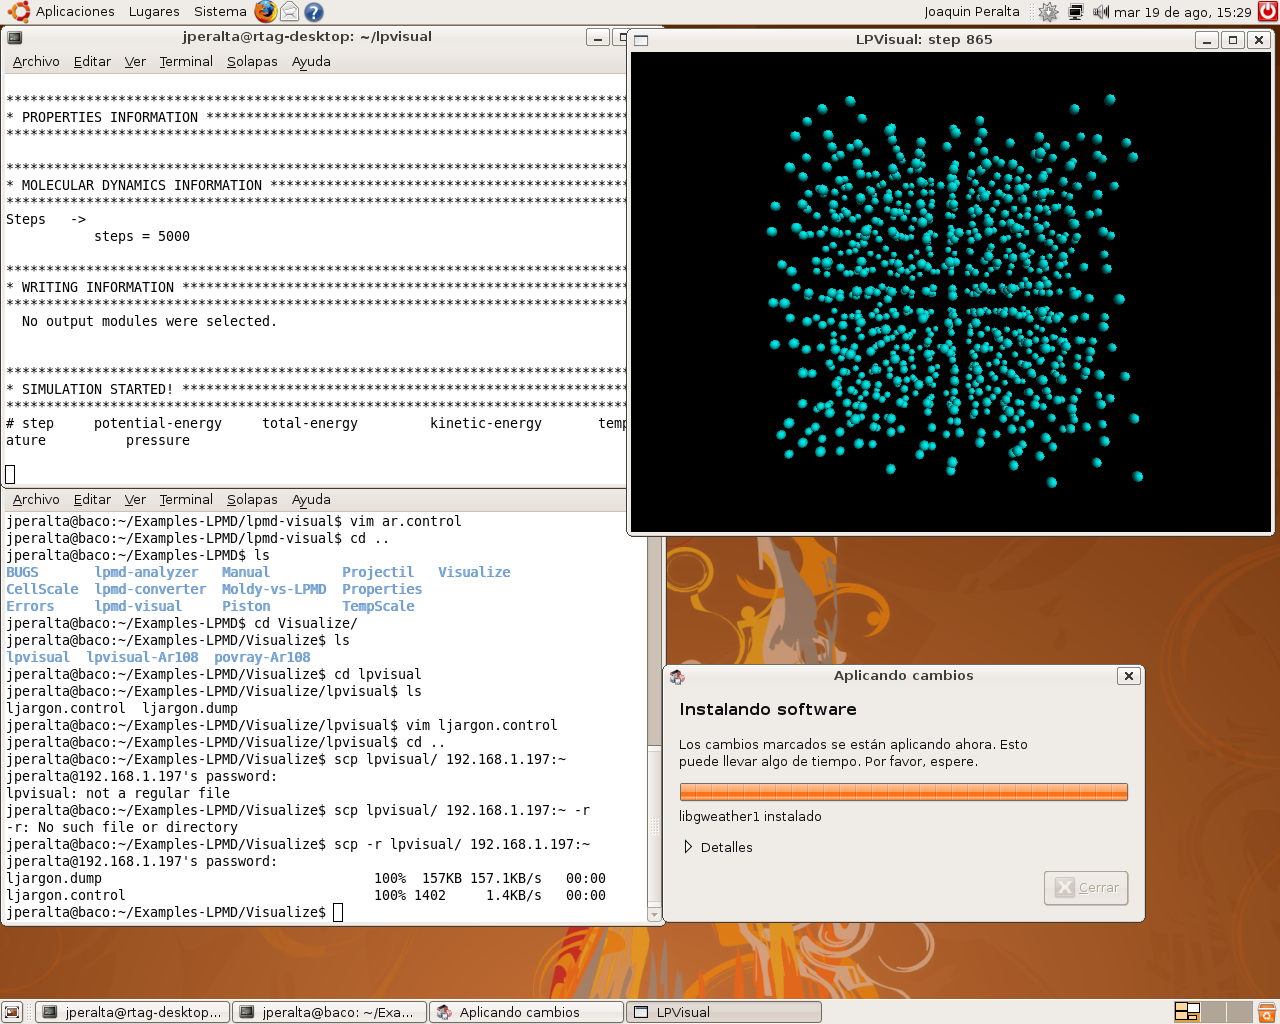
\includegraphics[scale=.25]{lpvisual.png}
 \label{fig:lpvisual}
 \caption{Screenshoot de \lpmd ejecutando una simulaci\'on de din\'amica molecular, mientras se observan las configuraciones en tiempo real con \textbf{lpvisual}.}
\end{figure}

Esta completamente basado en OpenGL, y el soporte es completamente independiente, cualqueir duda o consulta respecto al m\'odulo, contacte directamente al autor.

La descarga de \textbf{lpvisual}, se puede realizar a trav\'es de \verb|subversion|, con:

\control{svn co sn://www.gnm.cl/lpmd/lpvisual lpvisual}

Para la instalaci\'on y configuraci\'on refierase directamente a la documentaci\'on del m\'odulo.

\subsection{povray}
Genera diretorios con ficheros pov para visualizar el sistema. Este m\'odulo genera un set de archivos \verb|pov| los cuales son ubicados dentro de un directorio, para un posterior \textit{rendering} para el dise\'no de peliculas o fotograf\'ias de la simulaci\'on. Hasta la fecha el soporte y las caracteristicas del m\'odulo no son muy buenas, sin embargo espera mejorarse en proximas versiones.

Los argumentos requeridos por el m\'odulo povray, son los siguientes,

\cajatx{
\begin{tabular}{lcl}
 header & = & Es un nombre previo al nombre \\
&&de los ficheros \textbf{pov} que ser\'an generados.\\
 direct & = & Nombre del directorio que se crear\'a.\\
 text & = & Orden para poner texto en \\
&&diferentes posiciones.\\
 background & = & Color del fondo de la imagen. \\
 rotate & = & Orientaci\'on de la c\'amara.\\
 logo   & = & Si desea anadir una imagen. \\
 box  & = & Muestra o no la \textbf{celda} (True/False).\\
 camera & = & Posici\'on de la c\'amara \\
 &&(recomendamos default).\\
\end{tabular}
}

Dentro de cada uno de \'estos argumentos, el que m\'as cabe detallar es \textbf{text}, el formato de ingreso de textos para la visualizaci\'on, es el siguiente,

\control{text "Titulo" <pos> <color> [size] (extra)}

Ac\'a las opciones son en el orden requerido. El t\'itulo puede ser cualquier texto, si se utiliza el s\'imbolo ``\% '' entonces el valor de \verb|extra| ser\'a reemplazado (Actualmente : Temp, Step). Las opciones \verb|<pos>| y \verb|<color>| son vectores que deben ingresarse en el formato \verb|<x,y,z>| y corresponden a la posici\'on del texto y los colores, exiten valores por defecto, tales como \verb|<green>|, \verb|<red>| o posiciones como \verb|<dl>| (abajo a la izquierda) que pueden ser utilizadas. Finalmente [size] es el tama\~no escalado del texto. Para una visi\'on m\'as detallada revise el cap\'itulo~\ref{chap:exa}.

% A continuaci\'on un ejemplo t\'ipico de uso de \verb|povray| en una simulaci\'on.
% 
% \begin{verbatim}
% use povray
%     header shoot-
%     direct movie
%     text "Modelacion de Ar" <dl> <green> [1] ()
%     text "Step = %" <3,3,3> <red> [1] (Step)
%     text "Temperatura : % [K]" <uc> <blue> [1] (Temp)
%     text "http://www.gnm.cl/" <dr> <green> [0.5] ()
%     background <0.2,0.1,0.4>
%     rotate <0,0,0>
%     logo "logo-v2.gif" 1.5 <cr>
% enduse
% \end{verbatim}
% 
% Luego de que los archivos son creados en el directorio ``movie'', es importante que coloque en ese directorio el logo al que los archivos hacen referencia \verb|logo-v2.gif|.

%%%%%%%%%%%%%%%%%%%%%%%%%%%%%%%%%%%%%%%%%%%%%%%%%%%%%%%%%%%%%%%%%
%%%%%%%%%%%%%%%%%%%%%%%%%%%%%%%%%%%%%%%%%%%%%%%%%%%%%%%%%%%%%%%%%
\section{Propiedades Est\'aticas}
Las propiedades est\'aticas, son aquellas que se pueden evaluar en cualquier instante de tiempo, las que se listan a continuaci\'on, son las que se han implementado a la fecha.
\subsection{angdist}
Calcula la distribucion angular de la celda de simulaci\'on. Para determinar los \'angulos caracter\'isticos de una celda de simulaci\'on es necesario entender el esquema o preocedimiento:
\begin{enumerate}
 \item Se selecciona un \'atomo $i$.
 \item Se busca un \'atomo $j$ que se encuentre dentro del radio de corte $r_{ij}$
 \item Se busca un \'atomo $k$ que se enceuntre dentro del radio de corte $r_{ik}$
 \item Se calcula el \'angulo  $\angle j-i-k$ y se a\~nade en la cuenta
\end{enumerate}

De esta forma obtenemos una funci\'on entre 0 y 180$^\circ$ que nos muestra cuales son los principales angulos de ``enlace'' o ``distancia'' de los \'atomos. Las opciones de uso son:

\cajatx{
\begin{tabular}{lcl}
 bins & = & N\'umero de intervalos entre 0 y 180 grados. \\
 atoms & = & N\'umero de especies at\'omicas y los s\'imbolos\\
&&asociados a cada una.\\
 rcut & = & Se especifican 2 especies at\'omicas y su radio\\
&&de corte.\\
 output & = & Archivo de salida.\\
 average & = & Se promediar\'an o no los calculos.\\
\end{tabular}
}

\subsection{cordnum}
Calcula el n\'umero de cordinaci\'on de la celda, informandonos a modo de histograma, como se han encontrado los n\'umeros de vecinos asociados a la muestra. La manera de calcular este numero de coordinacion es:
\begin{enumerate}
 \item Se genera un arreglo entre 0 y el m\'aximo n\'umero de vecinos posibles.
 \item Para cada \'atomo $i$, se ve cuantos vecinos $j$ tiene dentro de un radio d corte $r_{ij}$.
 \item Se entrega un valor porcentual del conteo previo.
\end{enumerate}

\cajatx{
\begin{tabular}{lcl}
 maxn & = & N\'umero m\'aximo d vecinos para el histograma.\\
 atoms & = & N\'umero de especies at\'omicas y los s\'imbolos\\
&&asociados a cada una.\\
 rcut & = & Se especifican 2 especies at\'omicas y su radio\\
&&de corte.\\
 output & = & Archivo de salida.\\
 average & = & Se promediar\'an o no los calculos.\\
\end{tabular}
}


\subsection{cordnumfunc}
Calcula el n\'umero de cordinaci\'on de la celda, en este caso es la funci\'on m\'as usada n publicaciones, pero en ocaciones puede ser m\'as simple de analizar, el m\'etodo \textbf{cordnum}. Corresponde tambi\'en a la integraci\'on de la funci\'on de distribuci\'on de pares.
\begin{enumerate}
 \item Se selecciona una distancia m\'axima y se divide en intervalos.
 \item Se selecciona un \'atomo $i$.
 \item Se analiza cuantos atomos $j$ caen en la distancia asociada al intervalo.
 \item Se continua de forma acumulativa, hasta un valor rasonable.
\end{enumerate}

La forma de utilizar el m\'etodo esta dada por:

\cajatx{
\begin{tabular}{lcl}
 bins & = & N\'umero m\'aximo de intervalos entre 0 y \textbf{rcut}.\\
 atoms & = & N\'umero de especies at\'omicas y los s\'imbolos\\
&&asociados a cada una.\\
 rcut & = & Radio de corte m\'aximo para an\'alisis.\\
 output & = & Archivo de salida.\\
 average & = & Se promediar\'an o no los calculos.\\
\end{tabular}
}

\subsection{gdr}
Caulcula la funcion de distribucion de pares de la celda. Es uno de los m\'etodos utilizados para determinar las distancias principales a primeros y segundos vecinos de una celda de simulaci\'on. El procedimiento es el siguiente:
\begin{enumerate}
 \item Se selecciona un \'atomo $i$.
 \item Se ve cuantos atomos $j$ estan dentro de un cascar\'on esf\'erico centrado en $i$.
 \item Se promedia sobre los \'atomos asociados.
\end{enumerate}

\cajatx{
\begin{tabular}{lcl}
 bins & = & N\'umero m\'aximo de intervalos entre 0 y \textbf{rcut}.\\
 rcut & = & Radio de corte m\'aximo para an\'alisis.\\
 output & = & Archivo de salida.\\
 average & = & Se promediar\'an o no los calculos.\\
\end{tabular}
}

\subsection{densityprofile}
Calc\'ula un perfil de densidades bidimensional. Este m\'etodo divide la celda de simulaci\'on en cajas pequenas, en una direccion privilegiada y calcula las densidades en cada una de ellas, da una idea muy clara de la densidad ``por secci\'on'' de la celda de simulaci\'on.

La forma de utilizarla es:

\cajatx{
\begin{tabular}{lcl}
 axis & = & Valor del eje preferencial, o direcci\'on, del c\'alculo.\\
 bins & = & N\'umero de intervalos para dividir el eje.\\
 range & = & Rango espacial de cada uno de los ejes, con \\
 && formato: nombre del eje, m\'inimo y m\'aximo.\\
 output & = & Archivo de salida.\\
 average & = & Se promediar\'an o no los calculos.\\
\end{tabular}
}

\subsection{tempprofile}
Calc\'ula un perfil de temperaturas bidimensional. Al igual que el m\'etodo anterior, se divide la caja en celdas pequenas, en donde calculamos la temperatura de cada una de ellas.

La forma de utilizar esto es:

\cajatx{
\begin{tabular}{lcl}
 axis & = & Valor del eje preferencial, o direcci\'on, del c\'alculo.\\
 bins & = & N\'umero de intervalos para dividir el eje.\\
 range & = & Rango espacial de cada uno de los ejes, con formato:\\
&&nombre del eje, m\'inimo y m\'aximo.\\
 output & = & Archivo de salida.\\
 average & = & Se promediar\'an o no los calculos.\\
\end{tabular}
}

\subsection{veldist}
Muestra como estan distribuidas las velocidades del sistema. La salida es un histograma de velocidades. La forma de uso es:

\cajatx{
\begin{tabular}{lcl}
 bins & = & N\'umero de intervalos para dividir el histograma.\\
 output & = & Archivo de salida.\\
 average & = & Se promediar\'an o no los calculos.\\
\end{tabular}
}

\subsection{localpressure}

Calcula una presion local de la celda de simulaci\'on, para eso utiliza el stress de los \'atomo en cada ``sub-celda'', los valores entregados, recomendamos graficarlos con escala de colores para poder observar fen\'omenos. 

La forma de utilizar el plugin es:
\cajatx{
\begin{tabular}{lcl}
 rcut & = & Radio de corte.\\
 n$\alpha$ & = & Divisiones para cada eje ($\alpha=x,y,z$).\\
 output & = & Archivo de salida.\\
 average & = & Se promediar\'an o no los calculos.\\
\end{tabular}
}


%%%%%%%%%%%%%%%%%%%%%%%%%%%%%%%%%%%%%%%%%%%%%%%%%%%%%%%%%%%%%%%%%
%%%%%%%%%%%%%%%%%%%%%%%%%%%%%%%%%%%%%%%%%%%%%%%%%%%%%%%%%%%%%%%%%
\section{Propiedades Din\'amicas}
Las porpiedades din\'amicas, \textbf{no} pueden ser calculadas durante la simulaci\'ond e din\'amica molecular, ya que poseen correlaci\'on temporal en su an\'alisis, es por ello que estos m\'odulos no deben ser cargados en un fichero de control para \lpmd. Sin embargo estas propiedades pueden calcularase a partir de los ficheros de salida, tales como \verb|xyz| o \verb|lpmd|, utilizando \verb|lpmd-analyzer|.
\subsection{vacf}
Calcula la funci\'on de autocorrelaci\'on de velocidades de la celda. Por el momento el plugin esta en etapa de mejora y documentaci\'on.
\subsection{msd}
Calcula el desplazamiento cuadratico medio del sistema. Por el momento el plugin esta en etapa de mejora y documentaci\'on.
